\clearpage
\section{Aufbau}
\begin{figure}[h]
\begin{center}
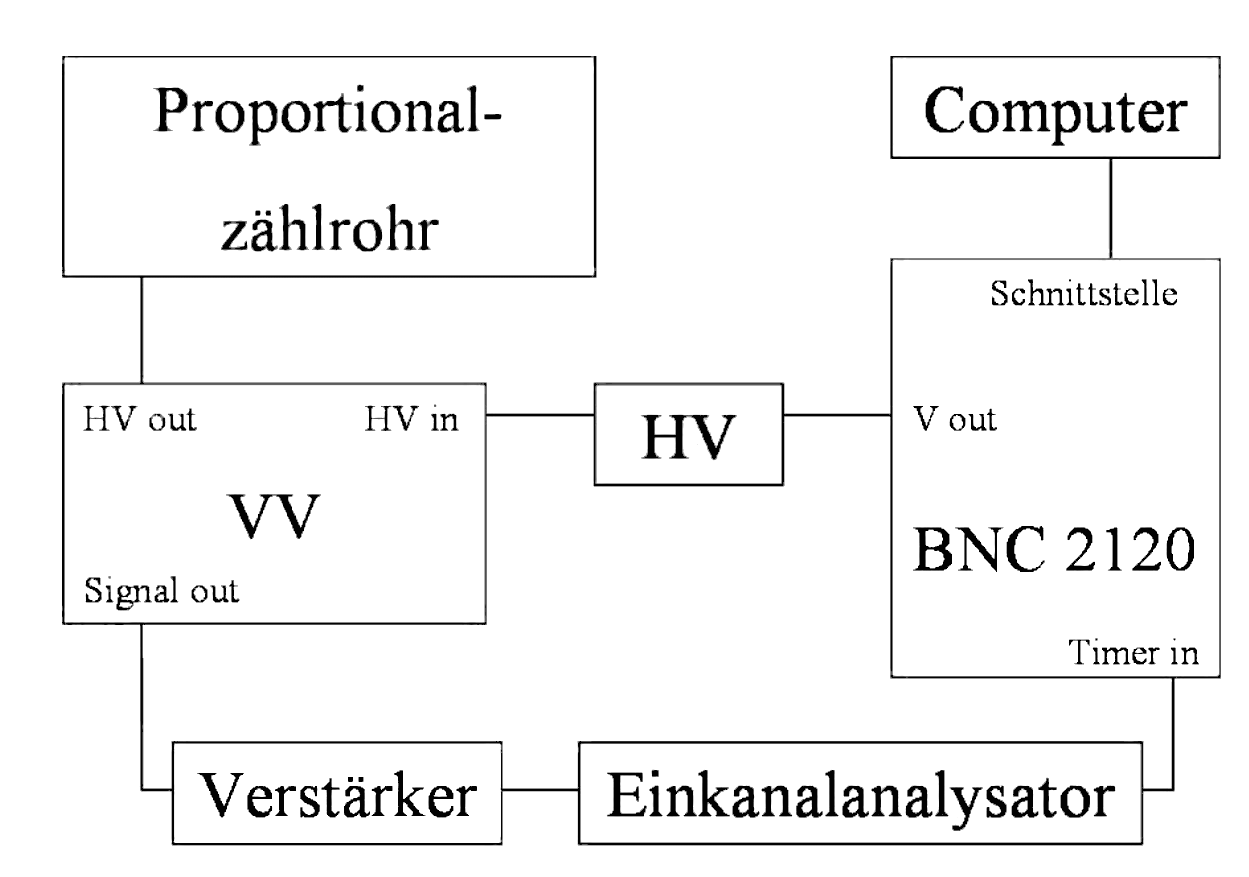
\includegraphics[scale=0.4]{Bilder/aufbau}
\caption{Versuchsaufbau, Quelle: [ver]}
\end{center}
\end{figure}
Die zu vermessenden Präparate werden mithilfe eines Drehtellers in das Methandurchflusszählrohr gebracht. Es kommt, wie bereits diskutiert, zur Wechselwirkung von Teilchen mit den Gasatomen, sodass Strompulse detektiert werden. Diese werden zum Vorverstärker ('VV') geleitet: Dieser wandelt die Strom- in Spannungspulse um und glättet sie. Die Hochspannung, welche am Zählrohr anliegt, wird vom Vorverstärker geliefert. Das Signal gelangt vom Vorverstärker zum Hauptverstärker ('HV'), wo es erneut zu einer Verstärkung kommt. Zudem kann hier die sogenannte 'Shaping Time' gewählt werden, welche die Zeitspanne angibt, über welche das Signal aufintegriert wird. An einem angeschlossenen Oszilloskop wird diese mitsamt des aufintegrierten, rechteckigen Signals angezeigt. Im darauffolgenden Einkanalanalysator wird eine untere Schranke ('lower level') eingestellt, welche die Mindestamplitude angibt, ab welcher ein Signal registriert wird. Mithilfe der 'Shaping Time' und der unteren Schranke können also statistische Schwankungen des Untergrunds herausgefiltert werden. Die registrierten Signale werden schließlich im Programm LabView am Computer durch die Messdauer geteilt: Auf diese Weise entsteht die Zählrate. Das Programm ermöglicht außerdem die Einstellung des zu vermessenden Spannungsintervalls, der Schrittweite, der Zeit, welche als Messdauer für jeden Spannungswert gewählt werden soll und der Zeit, welche dem Gerät gegeben werden soll, um sich auf eine Spannung einzupendeln.
\clearpage
\section{Durchführung}
Allgemein war zu beachten, dass bei Einführen der Probe in und Entfernen derselben aus dem Methandurchflusszählrohr das Gas ausgestellt ist. Bei den Messungen sollte das Gas aufgedreht sein, sodass man etwa 5 Bläschen/Sekunde am eingebauten Sichtfenster beobachten konnte. \\
Zunächst wurde die Zählrohrcharakteristik mithilfe einer Natururanprobe aufgenommen. Danach wurde ein Aluminiumschälchen mit KCl-Pulver unterschiedlicher Masse gefüllt und bei einer Arbeitsspannung, welche auf dem $\beta$-Plateau lag (s. 'Auswertung'), die Zählrate vermessen. Dies wurde für unterschiedliche Massen wiederholt. Schließlich wurde die Zählrate für das leere Aluminiumschälchen vermessen (Untergrund). \\
Dann sollte für die Samarium-Probe die Zählrate für unterschiedliche Oberflächen (hierfür lagen Aluminiumschälchen eingelassenen Oberflächen bereit) vermessen werden. Zunächst wurde das $\alpha$-Plateau aufgenommen, um einen Arbeitspunkt zu bestimmen. Dann wurde die untere Grenze so eingestellt, dass der Untergrund im Bereich von $0,3\frac{Counts}{s}$ lag. Schließlich wurde mithilfe eines Aluminiumschälchens und $Sm_{2}O_{3}$-Pulvers die Zerfallsrate vermessen. Als diese Messung fertig war, wurde ein mit Pulver gefülltes Schälchen anderer Oberfläche eingeführt. Dabei wurde eine vielfach höhere Zählrate gemessen. Auch ohne Probe und bei abgedrehtem Gas blieb diese Zählrate erhalten, was darauf schließen lässt, dass die Messung - vermutlich, da das Gerät sehr lange angeschaltet war - kein sinnvolles Ergebnis lieferte. Auch konnten auf dem Bildschirm des angeschlossenen Oszilloskops keine Signale beobachtet werden: Dennoch kam es zu detektierten Counts.